\documentclass[a4paper,12pt]{report}

\input{packages}
\input{styles}

\begin{document}

\input{names}

\thispagestyle{empty}

\begin{center}
Министерство образования и науки Российской Федерации \\ федеральное государственное бюджетное образовательное \\ учреждение высшего профессионального образования \\<<Сибирский государственный аэрокосмический университет \\ имени академика М.Ф. Решетнева>>
\end{center}

\vspace{20mm}

\vspace{30mm}
\begin{center}
{\large Сергиенко Антон Борисович}
\end{center}

\vspace{5mm}
\begin{center}
{\bf \large Генетический алгоритм. Стандарт. v.3.8
\par}

\vspace{10mm}

\vspace{10mm}

\end{center}

\vspace{80mm}

\vspace{20mm}
\begin{center}
{Красноярск -- 2013}
\end{center}

\newpage			% Титульный лист
\setstretch{0.9}

\tableofcontents

\singlespacing

\clearpage
		% Содержание
\chapter*{Условные обозначения}
\addcontentsline{toc}{chapter}{Условные обозначения}

$a \in A$ --- элемент $ a $ принадлежит множеству $ A $.

$ \bar{x} $ --- обозначение вектора.

$ \arg{f(x)} $ --- возвращает аргумент $x$, при котором функция принимает значение $ f(x) $.

$ Random(X) $ --- случайный выбор элемента из множества $ X $ с равной вероятностью.

$ Random\left ( \left \{x_i \mid p_i \right \} \right ) $ --- случайный выбор элемента $ x_i $ из множества $ X $, при условии, что каждый элемент $ x_i\in X $ имеет вероятность выбора равную $ p_i $.

$ Random\left ( \left \{x^i \mid p^i \right \} \right ) $ --- случайный выбор элемента $ x^i $ из множества $ X $, при условии, что каждый элемент $ x^i\in X $ имеет вероятность выбора равную $ p^i $, то есть это обозначение равнозначно предыдущему.

$ random(a,b) $ --- случайное действительное число из интервала $ [a; b] $.

$ int(a) $ --- целая часть действительного числа $ a $.

$ \mu(X) $ --- мощность множества $ X $.

$ \mathbb{N} $ --- множество натуральных чисел.

\textbf{Замечание.} Оператор присваивания обозначается через знак «$ = $», так же как и знак равенства.

\textbf{Замечание.} Индексация всех массивов в Стандарте начинается с $ 1 $. Это стоит помнить при реализации алгоритма на C-подобных языках программирования, где индексация начинается с нуля.

\textbf{Замечание.} Вызывание трех функций: $ Random(X) $, $ Random\left ( \left \{x_i \mid p_i \right \} \right ) $, $ random(a,b) $ – происходит каждый раз, когда по ходу выполнения формул, они встречаются. Если формула итерационная, то нельзя перед ее вызовом один раз определить, например, $ random(a,b) $ как константу и потом её использовать на протяжении всех итераций неизменной.

\textbf{Замечание.} Надстрочный индекс может обозначать как возведение в степень, так и индекс элемента. Конкретное обозначение определяется в контексте текста, в котором используется формула с надстрочным индексом.

\textbf{Замечание.} При выводе матриц и векторов элементы могут разделяться как пробелом, так и точкой с запятой, то есть обе записи $ {\left(\begin{array}{cccccccc}
 1&1&1&1&1&1&1&1
\end{array} \right)}^\mathrm{T} $ и $ {\left(1;1;1;1;1;1;1;1;1 \right)}^\mathrm{T} $ допустимы.

\textbf{Замечание.} При выводе множеств элементы разделяются только точкой с запятой, то есть допустима только такая запись: $ {\left\lbrace 1;1;1;1;1;1;1;1;1 \right\rbrace }^\mathrm{T} $.

\clearpage			% Условные обозначения
\chapter*{Введение}
\addcontentsline{toc}{chapter}{Введение}
\setstretch{0.95}
На данный момент генетический алгоритм (ГА) является одним из наиболее исследуемых и развивающихся алгоритмов глобальной оптимизации. К сожалению, до сих пор, по крайней мере, в российской литературе, строго описания алгоритма автором не встречалось. Обычно даны лишь общие рекомендации, которые допускают разночтение в процессе программирования. Либо предложенные схемы применимы лишь для решения тестовых задач. Из-за этого невозможно строго сопоставить друг другу различные исследования по эффективности алгоритмов. Как сказал один из исследователей: «Количество различных эволюционных алгоритмов совпадает с количеством исследователей, работающих в данной области!» \cite{web:makeingsimpleGA}. Данная работа призвана определить некий стандарт генетического алгоритма (далее Стандарт).

Данный документ представляет его версию 3.5 от \today

Последнюю версию документа можно найти по адресу:

\href{https://github.com/Harrix/Standard-Genetic-Algorithm}{https://github.com/Harrix/Standard-Genetic-Algorithm}

\textbf{Цель Стандарта} --- предоставить исследователям единое описание генетического алгоритма для последующей оценки и сравнения эффективности ГА и других алгоритмов. 

Задача, которую решает Стандарт --- определить технологию реализации сГА (стандартный генетический алгоритм). Технология обеспечивает единое понимание и одинаковую реализацию.

В качестве объекта в Стандарте выступает сГА однокритериальной оптимизации на бинарных или вещественных строках.

Стандарт предназначен, в первую очередь, для следующих пользователей:
\begin{itemize}
\item исследователей, занимающиеся  разработкой и исследованиями модификаций ГА (студенты, аспиранты, докторанты, любители-энтузиасты и др.);
\item экспертов, кто может участвовать в оценке результатов работ исследователей.
\end{itemize}


Автор выражает благодарности людям, помогающим в работе данного Стандарта: Бухтоярову Владимиру Викторовичу (\href{mailto:vladber@list.ru}{vladber@list.ru}), Галушину Павлу Викторовичу (\href{mailto:galushin\_pavel@mail.ru}{galushin\_pavel@mail.ru}), Семенкину Евгению Станиславовичу (\href{mailto:eugenesemenkin@yandex.ru}{eugenesemenkin@yandex.ru}), Сергиенко Роману Борисовичу (\href{mailto:romaserg@list.ru}{romaserg@list.ru}), Сопову Евгению Александровичу (\href{mailto:es\_gt@mail.ru}{es\_gt@mail.ru}), Сопову Сергею Александровичу (\href{mailto:sopov.sa@gmail.com}{sopov.sa@gmail.com}).

В данной версии документа по сравнению с предыдущем произведен перевод на \LaTeX\ систему и платформу GitHub, рисунки все переведены в векторный формат, исправлены ошибки и добавлены некоторые замечания.

С автором можно связаться по адресу \href{mailto:sergienkoanton@mail.ru}{sergienkoanton@mail.ru} или  \href{http://vk.com/harrix}{http://vk.com/harrix}.

Сайт автора, где публикуются последние новости: \href{http://blog.harrix.org/}{http://blog.harrix.org/}, а проекты располагаются по адресу \href{http://harrix.org/}{http://harrix.org/}.

\singlespacing
\clearpage	% Введение
\chapter{Постановка задачи оптимизации}\label{StandardGA:section_problemoptimization}

Рассмотрим постановку задачи оптимизации в общем случае, решаемую стандартным генетическим алгоритмом (сГА).

Необходимо найти:
\begin{equation}
\label{StandardGA:eq:problemoptimization}
\bar{x}_{max} = \arg{ \max_{\bar{x} \in X}{f\left ( \bar{x} \right )} }\text {, где}
\end{equation}
\begin{equation*}
g_i\left (\bar{x}\right )\leq 0, i=\overline{1,m_1},
\end{equation*}
\begin{equation*}
h_j\left (\bar{x}\right )= 0, j=\overline{1,m_2}.
\end{equation*}

Здесь:

$ X $ --- множество всех возможных решений,

$ f\left ( \bar{x} \right ) $ --- функционал, определенный на данном множестве, возвращающий действительное число из интервала $ (-\infty;\infty) $,

$ m_1 $ --- число ограничений в виде неравенств,

$ m_2 $ --- число ограничений в виде равенств.

$ \bar{x} \in X $ имеет вид 
\begin{equation}
\label{StandardGA:eq:formofvector}
\bar{x}={\left(x_1;\dots;x_i;\dots;x_n \right)}^\mathrm{T}.
\end{equation}

В случае, если $ m_1=0 $ и $ m_2=0 $, имеем задачу безусловной оптимизации. В противном случае --- условной оптимизации.

В случае, если $ X $ --- множество всех бинарных векторов длины $ n $ таких что $ x_i\in\left\lbrace 0;1\right\rbrace  (i\hmm=\overline{1,n})$, то имеем задачу бинарной оптимизации (мощность поискового пространства $ X $ равна $ \mu(X)=2^n $). Если $ X $ --- множество всех вещественных векторов длины $ n $ таких что $ x_i\in\left\lbrace Left_i;Right_i\right\rbrace (i=\overline{1,n}) $, то имеем задачу вещественной оптимизации.

Будем предполагать в дальнейшем, что $ f(\bar{x}) $ может представлять собой  многоэкстремальный функционал, и вычислению подлежат только значения $ f(\bar{x}) $ (нет возможности вычислить производные от функционала и т.~д.).

Стандартный генетический алгоритм, описанный в Стандарте, решает задачи оптимизации на бинарных и вещественных векторах. При решении задачи на вещественных строках происходит преобразования исходной задачи к задаче оптимизации на бинарной строках, на основе стандартного представление целого числа --- номера узла в сетке дискретизации или стандартным рефлексивным Грей-кодом.

\textbf{Пример.} Требуется найти бинарный вектор длины $ n=8 $, сумма компонент которого максимальна:
\begin{equation}
\label{StandardGA:eq:problemoptimizationexample}
 \bar{x}_{max} = \arg{ \max_{\bar{x} \in X}{f\left ( \bar{x} \right )} }\text {, где}
\end{equation}
\begin{equation*}
 f\left ( \bar{x} \right )=\sum_{i=1}^{n}x_i.
\end{equation*}

Очевидно, что $ \bar{x}_{max}={\left(1;1;1;1;1;1;1;1;1 \right)}^\mathrm{T} $, но алгоритм это «не знает», и его задача --- найти это решение.

\begin{figure} [h] 
  \center
  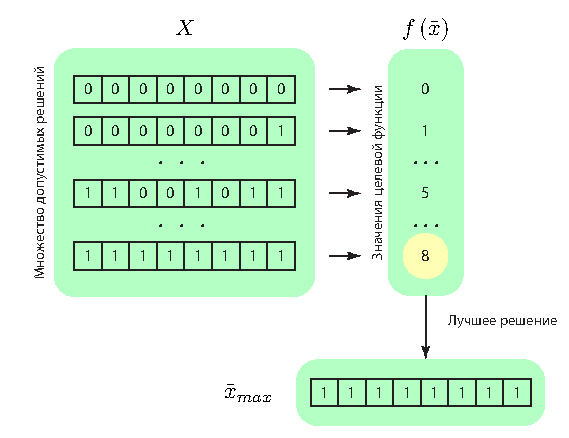
\includegraphics {ExampleProblemOptimization.pdf}
  \caption{Пример задачи оптимизации} 
  \label{StandardGA:img:ExampleProblemOptimization.pdf}  
\end{figure}


\clearpage			% Глава 1
\chapter{Определения генетического алгоритма}\label{StandardGA:section_def}

Введем некоторые понятия, которыми будем пользоваться в данном Стандарте.

\textbf{Стандартный генетический алгоритм} --- генетический алгоритм, описанный в данном документе. Он считается базовым для исследования эффективности других ГА. Если не оговорено иное, то под генетическим алгоритмом понимается стандартный генетический алгоритм. Для обозначения также используется сокращение сГА.

\textbf{Бинарная строка} --- вектор-столбец $\bar{x}$ конечной длины $ n $, компоненты которого могут принимать значения из множества $ \left\lbrace 0; 1\right\rbrace  $. В принципе не совсем верное название, так как по сути это вектор-столбец, а не вектор-строка.

\textbf{Бинарный вектор} --- то же самое, что и бинарная строка.

\textbf{Вещественная строка} --- вектор-столбец $\bar{x}$ конечной длины $ n $, компоненты которого могут принимать значения из множества $ x_i\in\left\lbrace Left_i;Right_i\right\rbrace (i=\overline{1,n}) $. По своей сути не совсем верное название, так как по сути это вектор-столбец, а не вектор-строка.

\textbf{Вещественный вектор} --- то же самое, что и вещественная строка.

\textbf{Решение} --- любой элемент $\bar{x}$ из множества $ X $.

\textbf{Точка поискового пространства} --- то же самое, что и решение.

\textbf{Возможное решение} --- любое решение $\bar{x}$ из множества $ X $.

\textbf{Допустимое решение} --- решение $\bar{x}$ из множество $ X $, которое удовлетворяет условиям $ g_i\left (\bar{x}\right )\leq 0 \left( i=\overline{1,m_1},\nonumber\right)  $ и $ h_j\left (\bar{x}\right )= 0 \left(  j=\overline{1,m_2}\right)  $.

\textbf{Генотип} --- то же самое, что и бинарная строка.

\textbf{Индивид} --- то же самое, что и бинарная строка. 

\textbf{Хромосома} --- то же самое, что и бинарная строка.

\textbf{Ген} --- компонент $ x_i $ бинарного вектора $\bar{x}\in X$.

\textbf{Бит} --- компонент $ x_i $ бинарного вектора $\bar{x}\in X$.

\textbf{Фенотип} --- некий объект, который был закодирован в бинарную, строку при переходе от задачи оптимизации на произвольном пространстве поиска к задаче оптимизации на бинарных строках. Например, вещественный вектор преобразуется в бинарную строку с помощью кода Грея.

\textbf{Поколение} --- одна итерация работы сГА.

\textbf{Популяция} --- множество индивидов, обрабатываемых на текущем поколении.

\textbf{Целевая функция} --- то же самое, что и функционал $ f\left( \bar{x}\right)  $.

\textbf{Оптимизируемая функция} --- то же самое, что и функционал $ f\left( \bar{x}\right)  $.

\textbf{Функция пригодности} --- преобразованная целевая функция для использования в генетическом алгоритме на бинарных строках.

\textbf{Пригодность} --- значение функции пригодности.

\textbf{Поисковое пространство} --- множество всех возможных векторов $ X $.

\textbf{Множество решений} --- то же самое что и поисковое пространство.

Остальные определения будут вводиться по мере их упоминания в тексте.

\textbf{Замечание.} Понятия «генотип», «хромосома», «индивид» обозначают по своей сути одно и то же. Но в связи с тем, что генетический алгоритм имитирует настоящую эволюцию, то на различных этапах имитации более подходящими являются разные понятия из биологии.

Также стоить отметить, что здесь эти понятия отождествляются с бинарной строкой, как возможным решением, а не любым решением из первоначальной задачи оптимизации (там могут присутствовать также вещественные строки). Это объясняется тем, что в описанном в Стандарте генетическом алгоритме на уровне операторов используются именно бинарные строки. А задача вещественной оптимизации решается путем сведения к задаче бинарной оптимизации путем дискретизации поискового пространства, операторов кодирования и декодирования. Но это не означает, что в других вариантах генетического алгоритма, не описанных в Стандарте, понятия «генотип», «хромосома», «индивид» будут отождествляться с бинарными строками.

\clearpage			% Глава 2
\chapter{Общая модель стандартного генетического алгоритма}\label{StandardGA:section_commonmodel}

Генетический алгоритм можно представить как некий стохастический оператор, который на выходе выдает \textbf{субоптимальное} решение $ \bar{x}_{submax} $ и значение функционала от этого решения $ f\left( \bar{x}_{submax}\right)  $. То есть мы можем записать, что

\begin{equation}
\label{StandardGA:eq:commommodelGA}
\left( \begin{array}{c} \bar{x}_{submax} \\ f\left( \bar{x}_{submax}\right)\end{array}\right)=GeneticAlgorithm\left( \begin{array}{c} X \\ f\left( \bar{x}\right) \\ g_i\left( \bar{x}\right) \\ h_j\left( \bar{x}\right) \\ Parameters \end{array}\right),
\end{equation}

где $i=\overline{1,m_1}, j=\overline{1,m_2}$,

$GeneticAlgorithm$ --- непосредственно сам генетический алгоритм как оператор,

$Parameters$ --- параметры генетического алгоритма, которые определяет пользователь (будут рассмотрены ниже).

В виде схемы это можно представить так:

\begin{figure} [h] 
  \center
  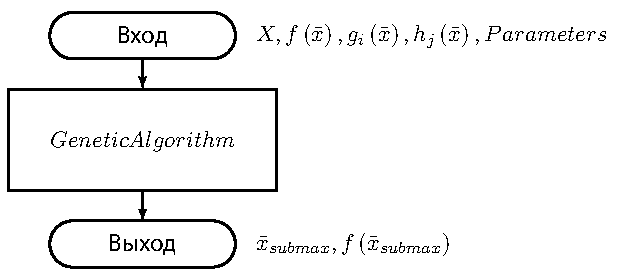
\includegraphics [scale=1] {GABlack}
  \caption{Модель черного ящика генетического алгоритма} 
  \label{StandardGA:img:GABlack}  
\end{figure}

Как было отмечено выше, стандартный генетический алгоритм (сГА) решает задачу оптимизации, как на бинарных строках, так и на вещественных. Поэтому стандартный генетический алгоритм включает в себя два алгоритма:

\begin{itemize}
\item стандартный генетический алгоритм на бинарных строках ($ BinaryGeneticAlgorithm $);
\item стандартный генетический алгоритм на вещественных строках.
\end{itemize}

При этом сГА на вещественных строках включает в себя сГА на бинарных строках, а также блок преобразования задачи вещественной оптимизации к задаче бинарной оптимизации и блок преобразования полученного бинарного решения к вещественному.

По этой причине вектор параметров сГА состоит из двух частей:

\begin{equation}
\label{StandardGA:eq:ParametersGA}
Parameters=\left( \begin{array}{c} ParametersOfBinaryGA \\ ParametersOfConvertingIntoBinaryGA\end{array}\right).
\end{equation}

Здесь $ ParametersOfBinaryGA $ --- параметры стандартного генетического алгоритма на бинарных строках, а $ ParametersOfConvertingIntoBinaryGA $ --- параметры преобразования задачи оптимизации на вещественных векторах к задаче оптимизации на бинарных векторах. В случае если в конкретном случае решается задача бинарной оптимизации, то блок параметров $ ParametersOfConvertingIntoBinaryGA $ можно опустить.

Построим общую схему сГА, учитывая вышесказанное (рис. \ref{StandardGA:img:GACommonSheme}).

\begin{figure} [h] 
  \center
  \includegraphics [scale=0.7] {GACommonSheme}
  \caption{Общая модель стандартного генетического алгоритма} 
  \label{StandardGA:img:GACommonSheme}  
\end{figure}

Распишем ее в виде алгоритма $ GeneticAlgorithm $:

\begin{algorithm}
\caption{Алгоритм $ GeneticAlgorithm $ (Часть 1)}\label{StandardGA:alg:GeneticAlgorithm}
\begin{algorithmic}

\State \textbf{Начало алгоритма}
\If{$ X $ представляет собой множество вещественных векторов}
\BeginBlock \parbox[t]{\dimexpr\linewidth-\algorithmicindent-\algorithmicindent-\algorithmicindent-\algorithmicindent-\algorithmicindent-\algorithmicindent}{\textbf{\textit{Преобразование задачи вещественной оптимизации в задачу бинарной оптимизации:}}\strut}
\State Выполнить:\begin{flalign*}
&\left( \begin{array}{c} X_{B} \\ f_B\left( \bar{x}_{B}\right)  \\ {g_i}_B\left( \bar{x}_B\right) \\ {h_j}_B\left( \bar{x}_B\right) \\ ParametersOfBinaryGA\end{array}\right)=\\
&=ConvertingIntoBinaryGA\left( \begin{array}{c} X \\ f\left( \bar{x}\right) \\ g_i\left( \bar{x}\right) \\ h_j\left( \bar{x}\right) \\ ParametersOfBinaryGA \\ ParametersOfConvertingIntoBinaryGA \end{array}\right);
\end{flalign*}
\EndBlock
\EndIf
\BeginBlock \parbox[t]{\dimexpr\linewidth-\algorithmicindent-\algorithmicindent-\algorithmicindent-\algorithmicindent-\algorithmicindent}{\textbf{\textit{Выполнение стандартного генетического алгоритма на бинарных строках:}}\strut}
\State \parbox[t]{\dimexpr\linewidth-\algorithmicindent}{Если решается задача бинарной оптимизации, то подается вектор входных параметров самого алгоритма $ GeneticAlgorithm $ (без $ ParametersOfConvertingIntoBinaryGA $, если он присутствует), иначе подается преобразованный вектор, полученный на предыдущем шаге:\strut}
\State $ A=\left\lbrace \begin{array}{l}
\left( \begin{array}{c} X \\ f\left( \bar{x}\right)  \\ {g_i}_B\left( \bar{x}\right) \\ {h_j}\left( \bar{x}\right) \\ ParametersOfBinaryGA\end{array}\right), \mbox{ где } X \mbox{ --- множество бинарных векторов};\\ 
\left( \begin{array}{c} X_{B} \\ f_B\left( \bar{x}_{B}\right)  \\ {g_i}_B\left( \bar{x}_B\right) \\ {h_j}_B\left( \bar{x}_B\right) \\ ParametersOfBinaryGA\end{array}\right), \mbox{ где } X  \mbox{ --- множество вещественных векторов.}
\end{array}\right. $

\State  $ \left( \begin{array}{c} \bar{x}{{}_{submax}}_B \\ {f\left( \bar{x}_{submax}\right)}_B \end{array}\right)=BinaryGeneticAlgorithm \left(  A \right)  $;
\EndBlock

\BeginBlock \textbf{\textit{Тип задачи:}}
\State Используем информацию, полученную на этапе «Анализ типа задачи»;
\If{$ X $ представляет собой множество вещественных векторов}
\State \Return ${\left( \bar{x}_{submax}; f\left( \bar{x}_{submax}\right) \right)}^\mathrm{T} $;
\EndIf
\EndBlock


\State \textit{Продолжение ниже}
  \algstore{bkbreak}
  
\end{algorithmic}
\end{algorithm}

\begin{algorithm}
\caption{Алгоритм $ GeneticAlgorithm $ (Часть 2)}
\begin{algorithmic}
\algrestore{bkbreak}
\State \textit{Начало выше}

\BeginBlock \textbf{\textit{Преобразование бинарного решения в вещественное:}}
\State $ \left( \begin{array}{c} \bar{x}_{submax} \\ f\left( \bar{x}_{submax}\right)\end{array}\right)=BinaryToReal \left( \begin{array}{c} \bar{x}{{}_{submax}}_B \\ {f\left( \bar{x}_{submax}\right)}_B \\ ParametersOfConvertingIntoBinaryGA \end{array}\right)  $;
\State \Return ${\left( \bar{x}_{submax}; f\left( \bar{x}_{submax}\right) \right)}^\mathrm{T} $;
\EndBlock


\State \textbf{Конец алгоритма}
\end{algorithmic}
\end{algorithm}

Операторы $ ConvertingIntoBinaryGA $ и $ BinaryToReal $ рассматриваются в главе \ref{StandardGA:section_realga}. До него рассматривается только стандартный генетический алгоритм на бинарных строках.

\textbf{Замечание.} Существует вещественный генетический алгоритм, который работает непосредственно с вещественными строками без приведения к задаче бинарной оптимизации. В данном Стандарте он не рассматривается.


\clearpage			% Глава 3
\chapter{Схема работы стандартного генетического алгоритма на бинарных строках}\label{StandardGA:section_shemebinaryGA}

В основу работы генетического алгоритма заложена имитация процесса эволюции живых организмов. Поэтому алгоритм представляет собой итерационный процесс (имитация смены поколений), работающий одновременно с несколькими взаимодействующими решениями (имитация популяции живых организмов).

Подробная схема, описывающая работу генетического алгоритма на бинарных строках ($ BinaryGeneticAlgorithm $), представлена ниже на рисунке.

\textbf{Замечание.} Довольно часто в литературе (например, \cite[с. 294]{book:Matveev2008}) рассматривается вариант, когда вначале отбираются потенциальные родители с помощью селекции (в «родительский пул»), а потом из них случайно отбираются родители для скрещивания. В данной модели генетического алгоритма это не происходит. Сразу после отбора двух родителей происходит скрещивание с целью получения одного потомка.

\begin{figure} [h] 
  \center
  \includegraphics [scale=0.8] {GABinarySheme}
  \caption{Схема генетического алгоритма на бинарных строках} 
  \label{StandardGA:img:GABinarySheme}  
\end{figure}


\clearpage			% Глава 4
\chapter{Описание стандартного генетического алгоритма на бинарных строках}\label{StandardGA:section_binaryGA}

Теперь приступим непосредственно к описанию самого алгоритма $ BinaryGeneticAlgorithm $ согласно схеме, приведенной выше.


\begin{algorithm}
\caption{Алгоритм $ BinaryGeneticAlgorithm $ (Часть 1)} \label{StandardGA:alg:BinaryGeneticAlgorithm}
\begin{algorithmic}
\State \textbf{Начало алгоритма}
\BeginBlock \textbf{\textit{Инициализация популяции:}}
\State $Population=Initialization\left( X\right) \text{, где } Population=\left\lbrace \bar{x}^1; \bar{x}^2; \ldots; \bar{x}^N \right\rbrace, \bar{x}^i \in X, i=\overline{1,N} $;
\EndBlock
\BeginBlock \textbf{\textit{Вычисление функции пригодности индивидов:}}
\State $Fitness=\left\lbrace f_{fit} \left( \bar{x}^1 \right); f_{fit} \left( \bar{x}^2 \right); \ldots; f_{fit} \left( \bar{x}^N \right) \right\rbrace $;
\EndBlock
\BeginBlock \textbf{\textit{Запоминание лучшего индивида и его значение целевой функции:}}
\State $\overline{Best}=\arg{ \max_{\bar{x} \in Population}{f\left ( \bar{x} \right )} }$;
\State $BestFitness=\max_{\bar{x} \in Population}{f\left ( \bar{x} \right )}$;
\EndBlock
\For{$M-1$ \textbf{раз}}
\For{\textbf{От }$j=1$ \textbf{до} $N$}
\BeginBlock \textbf{\textit{Селекция:}}
\State Выбрать двух родителей:
\State ${\overline{Parent}}^1=Selection\left( Population, Fitness, DataOfSel\right)$;
\State ${\overline{Parent}}^2=Selection\left( Population, Fitness, DataOfSel\right)$;
\State ${\overline{Parent}}^1\in X, {\overline{Parent}}^2\in X$;
\EndBlock
\BeginBlock \textbf{\textit{Скрещивание:}}
\State Получение потомка из родителей:
\State ${\overline{Child}}^j=Crossover\left({\overline{Parent}}^1,{\overline{Parent}}^2, DataOfCros\right)$;
\EndBlock
\EndFor
\BeginBlock \textbf{\textit{Мутация всех потомков:}}
\State Получение потомка из родителей:
\State \textit{Продолжение ниже}
\algstore{bkbreak}

\end{algorithmic}
\end{algorithm}
~\\

\begin{algorithm}
\caption{Алгоритм $ BinaryGeneticAlgorithm $ (Часть 2)}
\begin{algorithmic}
\algrestore{bkbreak}
\State \textit{Начало выше}
\State $MutChildPopulation=Mutation(ChildPopulation, DataOfMut),$
\State где $ChildPopulation=\left\lbrace {\overline{Child}}^1; \ldots; {\overline{Child}}^N\right\rbrace $, ${\overline{Child}}^i \in X$, $i=\overline{1,N}$;
\State $MutChildPopulation=\left\lbrace {\overline{MutChild}}^1; \ldots; {\overline{MutChild}}^N\right\rbrace $, ${\overline{MutChild}}^i \in X$, $i=\overline{1,N}$;
\EndBlock
\BeginBlock \textbf{\textit{Вычисление функции пригодности индивидов:}}
\State $FitnessOfMutChild=\left\lbrace f_{fit} \left( \overline{MutChild}^1 \right); f_{fit} \left( \overline{MutChild}^2 \right); \ldots; f_{fit} \left( \overline{MutChild}^N \right) \right\rbrace $;
\EndBlock
\BeginBlock \textbf{\textit{Запоминание лучшего индивида и его значение целевой функции:}}
\State \parbox[t]{\dimexpr\linewidth-\algorithmicindent-\algorithmicindent}{Если есть потомок лучше сохраненного лучшего индивида $\overline{Best}$, то заменяем его новым индивидом с его значением целевой функции:\strut}
\State $\overline{Best}=\arg{ \max_{\bar{x} \in MutChildPopulation \cup \overline{Best}}{f\left ( \bar{x} \right )} }$;
\State $BestFitness=\max_{\bar{x} \in MutChildPopulation \cup \overline{Best}}{f\left ( \bar{x} \right )}$;
\EndBlock
\BeginBlock \textbf{\textit{Формирование нового поколения:}}
\State \parbox[t]{\dimexpr\linewidth-\algorithmicindent-\algorithmicindent}{Из потомков и родителей формируется новое поколение, которое заменяет предыдущее поколение:\strut}
\State $\left( \begin{array}{c} NewPopulation \\ NewFitness \end{array}\right)=Forming\left( \begin{array}{c} Population \\ MutChildPopulation \\ Fitness \\ FitnessOfMutChild \\ DataOfForm \end{array}\right)$;
\State $Population=NewPopulation$;
\State $Fitness=NewFitness$;
\EndBlock
\EndFor
\BeginBlock \textbf{\textit{Выдаем лучшего индивида и его значение целевой функции:}}
\State \Return пару $\left( \begin{array}{c} \overline{Best} \\ BestFitness \end{array}\right)$. 
\EndBlock

\State \textbf{Конец алгоритма}
\end{algorithmic}
\end{algorithm}

Здесь,

$N$ --- размер популяции,

$M$ --- число поколений,

$ DataOfSel $ --- вектор параметров оператора селекции,

$ DataOfCros $ --- вектор параметров оператора скрещивания,

$ DataOfMut $ --- вектор параметров оператора мутации,

$ DataOfForm $ --- вектор параметров оператора формирования нового поколения.

При решении задачи нам известно количество вычислений целевой функции $ CountOfFitness $, которые мы можем реализовать. Данная величина определяется по затратам по вычислениям целевой функции в одной точке, временными ограничениями, экономической целесообразностью и другими причинами.

Вышеописанные переменные являются параметрами генетического алгоритма, варьируя которые мы получаем разные по эффективности реализации ГА. Во всех векторах параметров операторов главным параметром является тип данного оператора, так как существует несколько реализаций каждого из операторов.

При этом в сГА на бинарных строках число поколений и размер популяции берутся в таком соотношении, чтобы они были приблизительно одинаковыми. В таком случае мы можем исключить параметры $ M $ и $ N $ из числа определяемых пользователем, воспользовавшись формулой:

\begin{equation}
\label{StandardGA:eq:countM}
M=int \left( \sqrt{CountOfFitness}\right),
\end{equation}
\begin{equation*}
N=int \left( \dfrac{CountOfFitness}{M}\right).
\end{equation*}

Итак, определим вектор всех изменяемых параметров стандартного генетического алгоритма на бинарных строках:

\begin{equation}
\label{StandardGA:eq:ParametersOfBinaryGA}
ParametersOfBinaryGA=  \left( \begin{array}{c} CountOfFitness \\ DataOfSel \\ DataOfCros \\ DataOfMut \\ DataOfForm \end{array}\right).
\end{equation}

\textbf{Замечание.} В литературе часто в качестве критерия остановки алгоритма используется не число вычислений функции $ CountOfFitness $, а время работы алгоритма или достижение заданной точности задачи или самого алгоритма.

Если взять в качестве критерия время работы алгоритма, то исследования по сравнению алгоритмов будут жестко привязаны к компьютерам, на которых проводились вычисления. При этом критерий будет характеризовать скорее ЭВМ, чем алгоритм, и результаты будет сложно проверить другими исследователями. Следует помнить, что часто в практических задачах основное время работы занимает вычисление целевой функции, а не работы самого алгоритма, которое пренебрежительно мало.

Если же взять в качестве критерия остановки достижение заданной точности алгоритмом (например, $ K $ поколений проходят без улучшения наилучшего решения $ \overline{Best} $), то сравнивать между собой можно только эволюционные алгоритмы, так как данный критерий не приемлем для других алгоритмов глобальной оптимизации.

Использование в качестве критерия остановки достижение заданной точности задачи (например, расстояние до точки глобального оптимума) не содержит каких либо явных противоречий при исследованиях различных алгоритмов, но в данной работе не рассматривается.

\textbf{Замечание.} Число вычислений функций $ CountOfFitness $ желательно выбирать из квадратов целых чисел: $ 50^2 $, $ 100^2 $ и т.~д. Иначе настоящее число вычислений целевой функции будет меньше, чем $ CountOfFitness $.

\textbf{Замечание.} $ Population $, $ MutChildPopulation $, $ ChildPopulation $ не являются подмножествами множества $ X $, так как могут содержать одинаковые элементы, что противоречит определению подмножества.

\textbf{Замечание.} В главном цикле алгоритма число повторений равно $ M-1 $, так как первые $ M $ вычислений функции пригодности приходится на вычисление пригодности индивидов после инициализации популяции.

\textbf{Замечание.} При реализации алгоритма следует следить, чтобы число вычислений целевой функции равнялось $ CountOfFitness $. Часто встречаются реализации ГА, в которых целевая функция одного и того же индивида просчитывается несколько раз. Например, в схеме алгоритма для операторов селекции используется значения $ f_{fit} \left( \bar{x} \right)  $, а при запоминании $ BestFitness $ используется значение $ f\left( \bar{x} \right) $. Иногда пересчитывают целевую функцию для определения как $ BestFitness $  так и $ f_{fit} \left( \bar{x} \right)  $ (трехкратное увеличение вычислений целевой функции). Рекомендуется хранить два массива: один для значений $ f\left( \bar{x} \right) $, другой для $ f_{fit} \left( \bar{x} \right)  $, значения которого рассчитываются через первый массив. Данное замечание не касается модификации ГА, использующее хранение значение целевой функции для всех уже просчитанных индивидов, в которой прежде чем считать значение целевой функции индивид проверяют по базе.

\textbf{Замечание.} При запоминании лучшего индивида $ \overline{Best} $ и его значение функции пригодности в случае наступления ситуации, когда в популяции есть индивид с равной пригодностью, что и $ \overline{Best} $, не нужно замещать $ \overline{Best} $ этим индивидом. Замещение происходит только в случае, когда находится индивид с лучшей, чем у $ \overline{Best} $, пригодностью.

\clearpage			% Глава 5
\chapter{Описание операторов}\label{StandardGA:section_operatorsGA}

Рассмотрим подробно каждый из операторов генетического алгоритма из его описания.

\section{Инициализация популяции} \label{StandardGA:subsection_Initialization}

\textbf{Инициализация популяции} ---  процесс формирования случайного массива с фиксированным числом $N$ элементов из множества $X$. При этом должно выполняться условие, что для любых $\bar{x},\bar{y}\in X$ вероятности попадания в популяцию один или более раз одинаковы.

Итак, данный оператор определяется формулой:

\begin{equation}
\label{StandardGA:eq:Initialization}
Initialization\left( X \right) = \left\lbrace {\bar{x}}^1; {\bar{x}}^2; \ldots; {\bar{x}}^N \right\rbrace, {\bar{x}}^i=Random\left( X\right), {\bar{x}}^i \in X, i=\overline{1,N}.
\end{equation}

\textbf{Пример.} Допустим, решаем задачу из примера из формулы \ref{StandardGA:eq:problemoptimizationexample}. Зададим размер популяции $ N=6 $. Тогда в результате работы оператора инициализации мы можем получить популяцию:

\begin{equation*}
\label{StandardGA:eq:InitializationExample}
Population=\left\lbrace \begin{array}{c} {\left( 0; 0; 1; 1; 0; 1; 1; 1 \right) }^\mathrm{T} \\ {\left( 1; 0; 0; 0; 0; 0; 0; 0 \right) }^\mathrm{T} \\ {\left( 1; 0; 0; 1; 1; 1; 1; 0 \right) }^\mathrm{T} \\ {\left( 1; 1; 0; 1; 0; 1; 1; 1 \right) }^\mathrm{T} \\ {\left( 0; 0; 1; 0; 0; 1; 1; 0 \right) }^\mathrm{T} \\ {\left( 1; 0; 1; 1; 1; 1; 1; 1 \right) }^\mathrm{T} \end{array}\right\rbrace.
\end{equation*}

\begin{figure} [h] 
  \center
  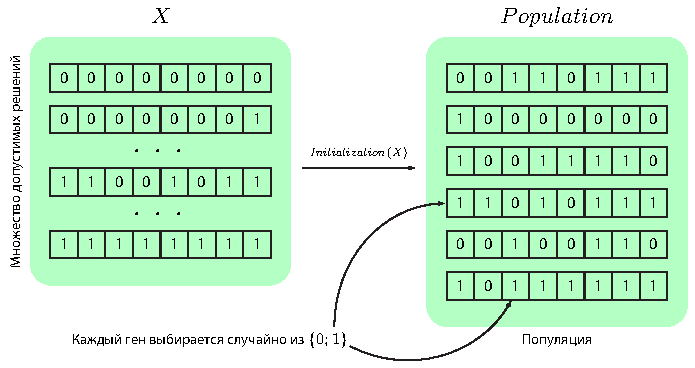
\includegraphics {Initialization.pdf}
  \caption{Инициализация популяции} 
  \label{StandardGA:img:Initialization.pdf}  
\end{figure}


\section{Вычисление функции пригодности} \label{StandardGA:subsection_fit}

Генетический алгоритм не работает с функционалом $ f\left(\bar{x} \right)  $, определяющий эффективность найденных решений. Как видно на схеме (рис. \ref{StandardGA:img:GABinarySheme}), ГА работает с функцией пригодности, которая для каждого индивида из популяции определяется по формуле:

\begin{equation}
\label{StandardGA:eq:fit}
f_{fit}\left( \bar{x}^k\right) = f_1 \left( f_2 \left( f\left( \bar{x}^k\right),g_i\left( \bar{x}^k\right),h_j\left( \bar{x}^k\right)\right),Y \right), 
\end{equation}
\indent где $\bar{x}^k \in Y$, $Y=Population \cup MutChildPopulation$, $k=\overline{1,N}$, $i=\overline{1,m_1}$, $j=\overline{1,m_2}$.

Запишем более кратко для простоты последующих выкладок:

\begin{align}
\label{StandardGA:eq:fitshort}
f_{fit}\left( \bar{x}^k\right) &\equiv f_1^k\left( f_2^k\right) \text{, где }\\
f_2^k&\equiv f_2 \left( f\left( \bar{x}^k\right),g_i\left( \bar{x}^k\right),h_j\left( \bar{x}^k\right)\right), \nonumber\\
f_1^k &\equiv f_1\left(f_2^k \right)\nonumber.
\end{align}

То есть значение функционала $ f\left( \bar{x}^k\right) $ претерпевает два преобразования.

$ f_2^k $ --- преобразование с учетом ограничений, накладываемых на задачу оптимизацию. Например, это может быть штрафы (смертельные, адаптивные и др.). В случае если $ m_1=0 $ и $ m_2=0 $ (задача безусловной оптимизации), то:

\begin{equation}
\label{StandardGA:eq:f_2^k}
f_2^k=f\left( \bar{x}^k\right), k=\overline{1,N}.
\end{equation}

$ f_1^k $ --- преобразование непосредственно по определению функции пригодности. Ее значение требуется в операторе селекции. При использовании пропорциональной селекции выдвигается требование, чтобы показатель эффективности решения был неотрицательной величиной. Функционал $f\left( \bar{x}\right)$ таким свойством не обладает. В литературе не описывается способов приведения к соответствующему виду $f\left( \bar{x}^k\right)$ (или точнее $ f_2^k $). Обычно сразу оговаривается, что $f\left( \bar{x}\right)$ ) обладает необходимыми условиями. Но тестовые функции, на которых проводятся исследования, этими свойствами не обладают. Из-за этого не адекватно сравнивать результаты исследования генетических алгоритмов. Например, при проверке одинаковых модификаций ГА у разных исследователей результаты могут отличаться, так как условия проведения экспериментов разные --- по своей сути решаются разные задачи оптимизации. Поэтому предлагается следующая формула, при использовании которой будет всегда выполняться условие $ f_1^k\geq 0 $:

\begin{equation}
\label{StandardGA:eq:f_1^k}
f_1^k=\left\lbrace \begin{aligned}
\dfrac{f_2^k-I^{min}}{I^{max}-I^{min}},\text { если } I^{max}\neq I^{min}; \\1 ,\text { если } I^{max}= I^{min}.
\end{aligned}\right.
\end{equation}
\begin{equation*}
I^{min}=\min_{\bar{x}^i \in Y} f_2^i, i=\overline{1,N};
\end{equation*}
\begin{equation*}
I^{max}=\max_{\bar{x}^i \in Y} f_2^i, i=\overline{1,N}.
\end{equation*}

\begin{figure} [h] 
  \center
  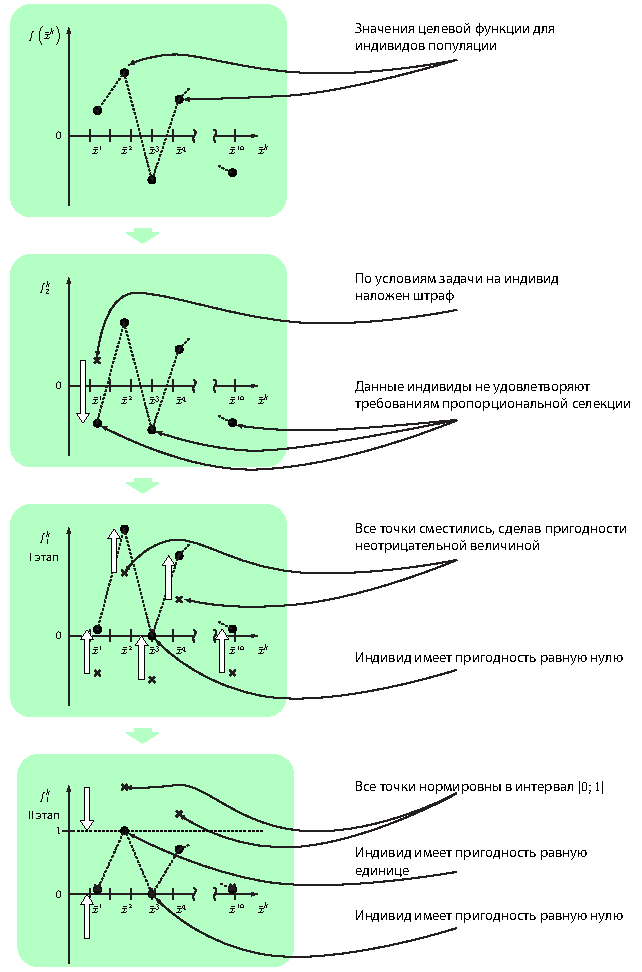
\includegraphics [scale=1] {Fitness}
  \caption{Пример получения пригодности индивидов популяции размера $N=10$} 
  \label{StandardGA:img:Fitness}  
\end{figure}

Отметим, что условие $ f_2^k\geq 0 $ не означает удовлетворения целевой функции требованиям пропорциональной селекции на всем множестве решений, так как условие рассматривает только решения из текущей популяции.

\textbf{Замечание.} Для других типов селекции (ранговая и турнирная) нет требования о неотрицательности функции пригодности. Но монотонное преобразование $ f_1^k $ не изменяет вероятности выбора индивидов из популяции ввиду того, что в данных типах селекции используется только попарное сравнение пригодностей, а не их численных значений.

\textbf{Замечание.} При преобразовании (\ref{StandardGA:eq:f_1^k}) обязательно найдется индивид с вероятностью выбора равной нулю в пропорциональной селекции. То есть в таком случае, всегда хотя бы один индивид в текущем поколении не имеет шансов стать родителем (кроме вырожденного случая, когда все поколение состоит из одного и того же индивида). Существуют другие преобразования $ f_1^k $, лишенные этого недостатка, но они не рассматриваются в данной работе.

\textbf{Замечание.} При использовании пропорциональной селекции  в случае, когда целевая функция (точнее ее преобразование с учетом ограничений) может принимать отрицательные значения, то пригодность одного и того же индивида может изменяться в разных поколениях из-за преобразования (\ref{StandardGA:eq:f_1^k}).

\textbf{Замечание.} Вычисления функции пригодности при программной реализации генетического алгоритма должны проводиться только на этапах «\textbf{Вычисление функции пригодности индивидов}». Во всех остальных операторах, если в формулах используется функция пригодности в виде $f\left( \bar{x}\right) $ или ином виде, то значения функции пригодности должны браться из сохраненных значений, а не расчитываться заново. В противном случае количество вычислений целевой функции не будет совпадать с тем, что задается для запуска генетического алгоритма.

\textbf{Замечание.} При программировании сГА на каком-нибудь языке программирования в качестве оптимизируемой функции можно подавать $ f_2^k $ ( то сеть целевая функция с учетом ограничений), а не полностью проработанную функцию пригодности. А дополнительные вычисления проводить внутри функции сГА, когда вызывается пропорциональная селекция.

\section{Селекция} \label{StandardGA:subsection_selection}

Селекция --- оператор случайного выбора одного индивида из популяции, основываясь на значениях функции пригодности всех индивидов текущей популяции, для использования его в операторе скрещивания. При этом вероятность выбора у индивидов с более высокой пригодностью выше, чем у индивидов с более низкой пригодностью.

В обычном генетическом алгоритме рассматривается три типа селекции, который определяется параметром $ TypeOfSelection $ из вектора $ DataOfSel $.

\textbf{Пропорциональная селекция.}
\begin{equation}
\label{StandardGA:eq:ProportionalSelection}
TypeOfSelection=ProportionalSelection.
\end{equation}

Вероятность выбора элемента пропорциональна значению пригодности индивида. Данный вид селекции может работать только с неотрицательными значениями пригодности, чем, и вызвано преобразование (\ref{StandardGA:eq:f_1^k}).

Пропорциональная селекция определяется формулой:

\begin{equation}
\label{StandardGA:eq:ProportionalSelection2}
Selection\left( Population, Fitness, DataOfSel\right) = Random\left( \left\lbrace\bar{x}^i | p^i \right\rbrace \right),
\end{equation}
\begin{equation}
p^i=\left\lbrace \begin{aligned}
\dfrac{f_{fit}\left( \bar{x}^i\right) }{\sum_{j=1}^N{f_{fit}\left( \bar{x}^j\right)}},&\text { если }  \exists f_{fit}\left( \bar{x}^k\right)\neq 0 \left( k=\overline{1,N} \right); \\ \dfrac{1}{N} ,&\text { иначе}.
\end{aligned}\right.
\end{equation}

где $ \bar{x}^i \in Population, i=\overline{1,N} $.

Как видим, формула определения вероятности выбора индивида имеет составной вид. Второе условие предназначено для маловероятного случая, когда в популяции все индивиды будут иметь пригодность равную нулю.

$ DataOfSel $ не содержит каких-либо параметров относительно данного типа селекции.

\textbf{Пример.} Пусть $ Fitness=\left\lbrace 0,5; 0,2; 0,1; 0,6; 0,2; 0,4\right\rbrace $. Тогда вероятности выбора индивидов равны:
\begin{flalign*}
p_1&=\frac{0,5}{0,5 + 0,2 + 0,1 + 0,6 + 0,2 + 0,4}=0,25;\\
p_2&=\frac{0,2}{0,5 + 0,2 + 0,1 + 0,6 + 0,2 + 0,4}=0,1;\\
p_3&=\frac{0,1}{0,5 + 0,2 + 0,1 + 0,6 + 0,2 + 0,4}=0,05;\\
p_4&=\frac{0,6}{0,5 + 0,2 + 0,1 + 0,6 + 0,2 + 0,4}=0,3;\\
p_5&=\frac{0,2}{0,5 + 0,2 + 0,1 + 0,6 + 0,2 + 0,4}=0,1;\\
p_6&=\frac{0,4}{0,5 + 0,2 + 0,1 + 0,6 + 0,2 + 0,4}=0,2.
\end{flalign*}

\begin{figure} [h] 
  \center
  \includegraphics [scale=0.7] {ProportionalSelection}
  \caption{Механизм работы пропорциональной селекции} 
  \label{StandardGA:img:ProportionalSelection}  
\end{figure}

\textbf{Ранговая селекция.}
\begin{equation}
\label{StandardGA:eq:RankSelection}
TypeOfSelection=RankSelection.
\end{equation}

Работает не  с массивом пригодностей напрямую, а массивом нормированных рангов, присваиваемых индивидам на основе значений пригодности. Используется функция, которая проставляет ранги для элементов несортированного массива пригодностей, то есть номера, начиная с $ 1 $, в отсортированном массиве. Если в массиве есть несколько одинаковых элементов, то ранги им присуждаются как среднеарифметические ранги этих элементов в отсортированном массиве. Если это не сделать, то вероятность выбора индивидов одинаковых по функции пригодности будет не равна друг другу, что противоречит идеи оператора селекции. Далее для выбора индивидов используется пропорциональная селекция, работающая с массивом рангов.

Значит, ранговая селекция определяется формулой:

\begin{equation}
\label{StandardGA:eq:RankSelection2}
Selection\left( Population, Fitness, DataOfSel\right) = Random\left( \left\lbrace\bar{x}^i | p^i \right\rbrace \right),
\end{equation}
\begin{equation}
p^i=\dfrac{Rank\left( f_{fit}\left( \bar{x}^i\right)\right)  }{\sum_{j=1}^N{Rank\left( f_{fit}\left( \bar{x}^j\right)\right)}},
\end{equation}
\begin{equation}\label{StandardGA:eq:Rank}
Rank\left( f_{fit}\left( \bar{x}^i\right)\right)=\dfrac{\sum_{j=1}^{N}{NumberOfSorting\left( f_{fit}\left( \bar{x}^i\right), Fitness\right)  \cdot S\left(  f_{fit}\left( \bar{x}^i\right),  f_{fit}\left( \bar{x}^j\right)\right) }}{\sum_{j=1}^{N}{S\left(  f_{fit}\left( \bar{x}^i\right),  f_{fit}\left( \bar{x}^j\right)\right) }},
\end{equation}
\begin{equation}
S\left(  f_{fit}\left( \bar{x}^i\right),  f_{fit}\left( \bar{x}^j\right)\right)= \left\lbrace \begin{array}{l}
1 \text{, если } f_{fit}\left( \bar{x}^i\right)=  f_{fit}\left( \bar{x}^j\right);\\ 0\text{, если } f_{fit}\left( \bar{x}^i\right)\neq  f_{fit}\left( \bar{x}^j\right).
\end{array}\right.
\end{equation}

где $ \bar{x}^i\in Population$, $i=\overline{1,N}.$

$NumberOfSorting\left( f_{fit}\left( \bar{x}^i\right), Fitness\right)$ --- функция, возвращающая номер элемента $ f_{fit}\left( \bar{x}^i\right)) $ в отсортированном массиве $ Fitness $ в порядке возрастания.

Формула (\ref{StandardGA:eq:Rank}) подсчитывает средние арифметические ранги при условии, что в массиве $ Fitness $  могут встречаться одинаковые элементы.

$ DataOfSel $ также не содержит каких-либо параметров относительно данного типа селекции.

\textbf{Пример.} Пусть $ Fitness=\left\lbrace 0,5; 0,2; 0,1; 0,6; 0,2; 0,4\right\rbrace $. Тогда вероятности выбора индивидов равны:
\begin{flalign*}
p_1&=\frac{5}{5+2,5+1+6+2,5+4}=0,238;\\
p_2&=\frac{2,5}{5+2,5+1+6+2,5+4}=0,119;\\
p_3&=\frac{1}{5+2,5+1+6+2,5+4}=0,047;;\\
p_4&=\frac{6}{5+2,5+1+6+2,5+4}=0,286;\\
p_5&=\frac{2,5}{5+2,5+1+6+2,5+4}=0,119;\\
p_6&=\frac{4}{5+2,5+1+6+2,5+4}=0,190.
\end{flalign*}

\begin{figure} [h] 
  \center
  \includegraphics [scale=0.8] {RankSelection}
  \caption{Механизм работы ранговой селекции} 
  \label{StandardGA:img:RankSelection}  
\end{figure}

\textbf{Турнирная селекция.}
\begin{equation}
\label{StandardGA:eq:TournamentSelection}
TypeOfSelection=TournamentSelection.
\end{equation}

Из популяции с равной вероятностью выбираются индивиды в количестве $ T $ (размер турнира), где $ 2\leq T\leq N $. При этом каждый индивид может попасть в группу (турнир) только один раз (турнирная селекция без возвращения). Из данной группы выбирается индивид с наибольшей пригодностью.

Значит, турнирная селекция определяется формулой:
\begin{align}
\label{StandardGA:eq:TournamentSelection2}
Selection\left( Population, Fitness, DataOfSel\right) = \arg{\max_{\bar{x}\in H} {f_{fit}\left( \bar{x}\right) }}, \text{где }\\
H=\left\lbrace h^i | h_i=Random \left( Population/\left( \left\lbrace h^1\right\rbrace \cup \left\lbrace h^2\right\rbrace \cup \ldots  \cup \left\lbrace h^{i-1}\right\rbrace\right) \right) \right\rbrace, i=\overline{1,T}\nonumber.
\end{align}

Турнирная селекция является единственным типом данного оператора, который добавляет в $ DataOfSel $ дополнительный параметр – размер турнира $ T $. Обычно выбирают значение этого параметра равное $ T=2 $.

\textbf{Пример.} Массив возьмем тот же, что и в предыдущих примерах $ Fitness=\left\lbrace 0,5; 0,2; 0,1; 0,6; 0,2; 0,4\right\rbrace $. Размер турнира равен $ T=3 $. Пример работы оператора показан на рисунке:

\begin{figure} [h] 
  \center
  \includegraphics [scale=0.8] {TournamentSelection}
  \caption{Механизм работы турнирной селекции} 
  \label{StandardGA:img:TournamentSelection}  
\end{figure}

Итак, мы рассмотрели используемые варианты селекции. Тогда можно составить вектор параметров оператора селекции $ DataOfSel $:

\begin{equation}
\label{StandardGA:eq:DataOfSel}
DataOfSel=\left( \begin{array}{c} TypeOfSel \\ T \end{array} \right).
\end{equation}

\textbf{Замечание.} Часто в литературе наряду с рассмотренными ниже тремя видами селекции упоминается элитарная селекция (элитная селекция, селекция элитизма). Этот оператор не является селекцией по определению этого оператора. В стандарте включен в состав одного из вида оператора формирования нового поколения из родителей и потомков.

\textbf{Замечание.} Часто при программировании турнирной селекции реализуется такой вариант, при котором один и тот же индивид из популяции может быть выбран в турнир несколько раз. Это происходит из-за простоты программирования данного способа, но является недопустимым при реализации вышеупомянутой селекции. В противном случае мы получаем модифицированный вариант турнирной селекции с возвращением, который требует дополнительных исследований.

Разумеется, выбранный индивид для участия в турнире, может принять участие в других турнирах.

\textbf{Замечание.} Часто в литературе встречаются различные варианты ранговой селекции, связанные с преобразованием значений рангов (возведение в квадрат и др.) В данной работе эти варианты не рассматриваются.

\textbf{Замечание.} Программировать оператор селекции рекомендуется таким образом, чтобы он возвращал не индивида, а его номер в популяции.

\textbf{Замечание.} Если при выполнении селекции сравниваются два разных индивида с одинаковыми значениями функций пригодности, то выбирается первый из них.

\section{Скрещивание} \label{StandardGA:subsection_Crossover}

\textbf{Скрещивание (кроссовер)} --- оператор случайного формирования нового индивида из двух выбранных родителей с сохранением признаков обоих родителей.

В обычном генетическом алгоритме рассматривается три типа скрещивания, который определяется параметром $ TypeOfCrossover $ из вектора $ DataOfCros $.

\textbf{Одноточечное скрещивание.}
\begin{equation}
\label{StandardGA:eq:SinglepointCrossover}
TypeOfCrossover=SinglepointCrossover.
\end{equation}

Пусть имеется два родителя (родительские хромосомы) $ \overline{Parent}^1 $ и $ \overline{Parent}^2$. В случайном месте происходит разрыв между двумя позициями генов в обеих хромосомах. После этого хромосомы обмениваются частями, в результате чего образуются два потомка. Из них выбирается случайно один потомок, который и передается в качестве результата оператора скрещивания. То есть скрещивание происходит по формулам:

\begin{align}
\label{StandardGA:eq:SinglepointCrossover2}
&Crossover \left( \overline{Parent}^1, \overline{Parent}^2, DataOfCros\right)=Random \left(\left\lbrace \overline{Offspring}^1; \overline{Offspring}^2\right\rbrace  \right), \\
&R=Random\left( \left\lbrace 2; 3; \ldots; n\right\rbrace \right); \nonumber \\
& \overline{Offspring}^1_i=\overline{Parent}^1_i, i=\overline{1,R-1};\nonumber\\
&  \overline{Offspring}^1_i=\overline{Parent}^2_i, i=\overline{R,n};\nonumber\\
&\overline{Offspring}^2_i=\overline{Parent}^2_i, i=\overline{1,R-1};\nonumber\\
& \overline{Offspring}^2_i=\overline{Parent}^1_i, i=\overline{R,n};\nonumber\\
&\overline{Offspring}^1\in X, \overline{Offspring}^2\in X.\nonumber
\end{align}

$ DataOfCros $ не содержит каких-либо параметров относительно данного типа скрещивания.

\textbf{Пример.} Для всех видов скрещивания будем использовать двух родителей: $\overline{Parent}^1\hm={\left( 0; 1; 0; 1; 1; 1; 0; 0\right)}^\mathrm{T}  $ и $\overline{Parent}^2={\left( 1; 1; 0; 0; 1; 0; 1\right)}^\mathrm{T}  $. Одноточечное скрещивание показано на рисунке:

\begin{figure} [h] 
  \center
  \includegraphics [scale=0.8] {SinglepointCrossover}
  \caption{Механизм работы одноточечного скрещивания} 
  \label{StandardGA:img:SinglepointCrossover}  
\end{figure}

\textbf{Двухточечное скрещивание.}
\begin{equation}
\label{StandardGA:eq:TwopointCrossover}
TypeOfCrossover=TwopointCrossover.
\end{equation}

Пусть имеется два родителя (родительские хромосомы) $\overline{Parent}^1$ и $\overline{Parent}^2$. В двух случайных местах происходят разрывы между двумя позициями генов в обеих хромосомах. После этого хромосомы обмениваются частями, в результате чего образуются два потомка. Из них выбирается случайно один потомок, который и передается в качестве результата оператора скрещивания. То есть скрещивание происходит по формулам:

\begin{align}
\label{StandardGA:eq:TwopointCrossover2}
&Crossover \left( \overline{Parent}^1, \overline{Parent}^2, DataOfCros\right)=Random \left(\left\lbrace \overline{Offspring}^1; \overline{Offspring}^2\right\rbrace  \right), \\
&r_1=Random\left( \left\lbrace 2; 3; \ldots; n\right\rbrace \right); \nonumber \\
&r_2=Random\left( \left\lbrace 2; 3; \ldots; n\right\rbrace \right); \nonumber \\
&R_1=\min \left( r_1, r_2\right) ; \nonumber \\
&R_2=\max \left( r_1, r_2\right) ; \nonumber \\
& \overline{Offspring}^1_i=\overline{Parent}^1_i, i=\overline{1,R_1-1};\nonumber\\
& \overline{Offspring}^1_i=\overline{Parent}^2_i, i=\overline{R_1,R_2-1};\nonumber\\
&  \overline{Offspring}^1_i=\overline{Parent}^1_i, i=\overline{R_2,n};\nonumber\\
& \overline{Offspring}^2_i=\overline{Parent}^2_i, i=\overline{1,R_1-1};\nonumber\\
& \overline{Offspring}^2_i=\overline{Parent}^1_i, i=\overline{R_1,R_2-1};\nonumber\\
&  \overline{Offspring}^2_i=\overline{Parent}^2_i, i=\overline{R_2,n};\nonumber\\
&\overline{Offspring}^1\in X, \overline{Offspring}^2\in X.\nonumber
\end{align}

$ DataOfCros $ не содержит каких-либо параметров относительно данного типа скрещивания.

\textbf{Пример.} Двухточечное скрещивание показано на рисунке:

\begin{figure} [h]
  \center
  \includegraphics [scale=0.8] {TwopointCrossover}
  \caption{Механизм работы двухточечного скрещивания} 
  \label{StandardGA:img:TwopointCrossover}  
\end{figure}

\textbf{Равномерное скрещивание.}
\begin{equation}
\label{StandardGA:eq:UniformCrossover}
TypeOfCrossover=UniformCrossover.
\end{equation}

Пусть имеется два родителя (родительские хромосомы) $\overline{Parent}^1$ и $\overline{Parent}^2$. Потомок состоит из генов, каждый из которых выбран случайно из генов родителей на соответствующих позициях. То есть скрещивание происходит по формулам:

\begin{align}
\label{StandardGA:eq:UniformCrossover2}
&Crossover \left( \overline{Parent}^1, \overline{Parent}^2, DataOfCros\right) = \overline{Offspring};\\
& \overline{Offspring}_i=Random\left( \left\lbrace \overline{Parent}^1_i;\overline{Parent}^2_i\right\rbrace \right), i=\overline{1,n} ;\nonumber\\
&\overline{Offspring}\in X.\nonumber
\end{align}

$ DataOfCros $ не содержит каких-либо параметров относительно данного типа скрещивания.

\textbf{Пример.} Равномерное скрещивание показано на рисунке:

\begin{figure} [h]
  \center
  \includegraphics [scale=0.7] {UniformCrossover}
  \caption{Механизм работы равномерного скрещивания} 
  \label{StandardGA:img:UniformCrossover}  
\end{figure}

Итак, мы рассмотрели используемые варианты скрещивания. Тогда можно составить вектор параметров оператора скрещивания $ DataOfCros $:

\textbf{Равномерное скрещивание.}
\begin{equation}
\label{StandardGA:eq:DataOfCros}
DataOfCros=\left( TypeOfCros\right) .
\end{equation}

\textbf{Замечание.} В одноточечном и двухточечном скрещивании разрыв хромосомы может произойти только между двумя генами, то есть в начале или конце хромосомы разрыв произойти не может, что является частой ошибкой при программировании. Такая операция не даст новых решений.

\textbf{Замечание.} В литературе присутствует два подхода к оператору скрещивания. Согласно первому в результате скрещивания получаются два потомка, которые оба попадают в популяцию потомков. Но этот способ накладывает ограничение на размер популяции $ N $: он должен быть четным. В данной работе используется второй подход, согласно которому в популяцию потомков попадает только один потомок, отобранный случайно. Есть варианты  в литературе, когда отбирается потомок с наилучшей пригодностью, но это в два раза увеличивает число вычислений функции, причем половина из них идет на вычисление функции пригодности индивидов, которые не примут участие в существовании популяции.

\textbf{Замечание.} В качестве двух родителей может выбраться один и тот же индивид $ \overline{Parent}^1\hm= \overline{Parent}^2 $. Это не запрещается в отличие от запрета попадания одного и того же индивида в турнир в турнирной селекции.

\textbf{Замечание.} В литературе в качестве одного из параметров скрещивания выступает вероятность скрещивания. Но часто она принимается за единицу, а многими исследователями вовсе опускается. В Стандарте (здесь описывается простейший вариант генетического алгоритма) данный параметр опущен.

Вероятность скрещивания меньше $ 1 $ исполняет роль операции клонирования. Хотя в Стандарте мы ее опустили, клонирование выполняется за счет селекции с повторением, то есть возможна реализация скрещивания одинаковых решений (см. предыдущее замечание)  --- аналог клонирования с очень низкой вероятностью.

\textbf{Замечание.} В двухточечном скрещивании точки разрыва могут совпасть. Тогда потомок будет совпадать с одним из родителей.

\textbf{Замечание.} Обратите внимание, что при описании оператора скрещивания для обозначения потомков используются $ \overline{Offspring} $, в схеме работы стандартного генетического алгоритма на бинарных строках $ \overline{Child} $. Это объясняется следующим образом. $ \overline{Child} $ используется для обозначения итогового потомка, который является результатом оператора скрещивания, тогда как $ \overline{Offspring} $ служит для обозначения временного потомка внутри работы оператора, и временных потомков может получиться несколько. Один из них, который выбирается, как описано выше, и становится возвращаемым $ \overline{Child} $.

\section{Мутация} \label{StandardGA:subsection_Mutation}

\textbf{Мутация} --- оператор случайного изменения всех потомков из популяции. Цель данного оператора  не получить более лучшее решение, а разнообразить многообразие рассматриваемых индивидов. Обычно мутация предполагает незначительное изменение потомков. При выполнении оператора каждый ген каждого индивида с некоторой заданной вероятностью  $ ProbabilityOfMutation $ мутирует, то есть меняет свое значение на противоположное. Мутация происходит по формулам:
\begin{align}
\label{StandardGA:eq:Mutation}
&\overline{MutChild}_j^i=\left\lbrace \begin{aligned}
\overline{Child}_j^i&\text{, если } random \left(0, 1 \right)>ProbabilityOfMutation; \\
1-\overline{Child}_j^i&\text{, иначе }.
\end{aligned}\right.\\
&\overline{Child}^i \in ChildPopulation, i=\overline{1,N},\nonumber\\
&\overline{MutChild}^i \in X, i=\overline{1,N}.\nonumber
\end{align}

Обычно в генетическом алгоритме вероятность мутации выбирается из трех вариантов: слабая ($ Weak $), средняя ($ Average $) и сильная ($ Strong $) мутация.
Отсюда вероятность мутации определяется формулой:
\begin{align}
\label{StandardGA:eq:ProbabilityOfMutation}
ProbabilityOfMutation\left( TypeOfMutation\right) =\\ =\left\lbrace \begin{aligned}
\frac{1}{3n}&\text{, если }TypeOfMutation=Weak; \\ \frac{1}{n}&\text{, если }TypeOfMutation=Average; \\ min\left(1, \frac{3}{n}\right) &\text{, если }TypeOfMutation=Strong.
\end{aligned}\right.\nonumber
\end{align}

Здесь
\begin{equation}
\label{StandardGA:eq:TypeOfMutation}
TypeOfMutation \in \left\lbrace Weak; Average;Strong\right\rbrace ,
\end{equation}

$ n $ --- длина вектора $ \bar{x}\in X $ бинарной задачи оптимизации.

Составим вектор параметров оператора мутации $ DataOfMut $:
\begin{equation}
\label{StandardGA:eq:DataOfMut}
DataOfMut=\left( TypeOfMutation\right) .
\end{equation}

\textbf{Замечание.} Определение сильной мутации через $ min\left(1, \frac{3}{n}\right) $  связано с тем, что при  $ n<3 $ вероятность мутации становится больше $ 1 $, что недопустимо. Но при программировании это не вызывает отклонений в работе генетического алгоритма, к тому же использование ГА для столь малых размерностей нецелесообразно.

\textbf{Замечание.} Часто в литературе под мутацией понимается не оператор над всеми потомками, а оператор над каждым в отдельности. Никакой принципиальной разницы в двух этих подходах нет.

\textbf{Пример.} На риc. \ref{StandardGA:img:Mutation} показана мутация одного из индивидов из популяции.

\begin{figure} [h]
  \center
  \includegraphics [scale=0.7] {Mutation}
  \caption{Механизм работы мутации} 
  \label{StandardGA:img:Mutation}  
\end{figure}

\section{Формирование нового поколения} \label{StandardGA:subsection_GenerationForming}

\textbf{Формирование нового поколения} --- оператор формирования нового поколения из массива родителей и получившихся потомков с использованием уже известных значений функции пригодности, как родителей, так и потомков.

В обычном генетическом алгоритме используется два типа формирования нового поколения, который определяется параметром $ TypeOfGenerationForming $ из вектора $ DataOfForm $.

\textbf{Только потомки.}
\begin{equation}
\label{StandardGA:eq:OnlyOffspringGenerationForming}
TypeOfGenerationForming=OnlyOffspringGenerationForming.
\end{equation}

Данная схема предполагает формирование нового поколения из потомков и родителей таким, что в новое поколение попадают только потомки. Данный тип формирования нового поколения определяется формулой:
\begin{equation}
\label{StandardGA:eq:OnlyOffspringGenerationForming2}
Forming \left( \begin{array}{c} Population\\MutChildPopulation\\Fitness\\FitnessOfMutChild\\DataOfForm\end{array}\right) =\left( \begin{array}{c} MutChildPopulation\\FitnessOfMutChild\end{array}\right).
\end{equation}

$ DataOfForm $ не содержит каких-либо параметров относительно данного типа формирования нового поколения.

\textbf{Только потомки и копия лучшего индивида.}
\begin{equation}
\label{StandardGA:eq:OnlyOffspringWithBestGenerationForming}
TypeOfGenerationForming=OnlyOffspringWithBestGenerationForming.
\end{equation}

Данная схема предполагает формирование нового поколения из потомков и родителей таким, что в новое поколение попадают только потомки (без одного) и копия лучшего индивида $ \overline{Best} $ (лучшего за всё время работы генетического алгоритма, а не только текущего поколения). В русской литературе данный способ часто называют селекцией элитизма. Данный тип формирования нового поколения определяется формулой:

\begin{align}
\label{StandardGA:eq:OnlyOffspringWithBestGenerationForming2}
&Forming \left( \begin{array}{c} Population\\MutChildPopulation\\Fitness\\FitnessOfMutChild\\DataOfForm\end{array}\right) =\left( \begin{array}{c} \left\lbrace \bar{x}^i\right\rbrace \\\left\lbrace f^i\right\rbrace\end{array}\right),\\&\bar{x}^i=\left\lbrace \begin{aligned}
\overline{Best}&\text{, если }i=0; \\ \overline{MutChild}^i&\text{, если }i\neq 0;
\end{aligned}\right.\nonumber\\
&f_i=f\left( \bar{x}_i\right), i=\overline{1,N}.\nonumber
\end{align}

$ DataOfForm $ не содержит каких-либо параметров относительно данного типа формирования нового поколения.

Итак, мы рассмотрели используемые варианты формирования нового поколения. Составим вектор параметров оператора формирования нового поколения:
\begin{equation}
\label{StandardGA:eq:DataOfForm}
DataOfForm=\left( TypeOfForm\right) .
\end{equation}

\clearpage			% Глава 6
\chapter{Решение задачи оптимизации на вещественных строках с помощью сГА}\label{StandardGA:section_realga}

До данной главы рассматривался стандартный генетический алгоритм на бинарных строках, который является составной частью сГА $ GeneticAlgorithm $. В случае, когда решается задача вещественной оптимизации, добавляются операторы преобразования задачи вещественной оптимизации в задачу бинарной оптимизации ($ ConvertingIntoBinaryGA $) и преобразования бинарного решения в вещественное ($ BinaryToReal $) (Алгоритм \ref{StandardGA:alg:GeneticAlgorithm}). При этом к вектору параметров сГА добавляется блок $ ParametersOfConvertingIntoBinaryGA $.

Существует различные реализации данных операторов. В Стандарте рассматривается два из них:
\begin{itemize}
\item стандартное представление целого числа --- номер узла в сетке дискретизации;
\item стандартный рефлексивный Грей-код.
\end{itemize}

Применяемый тип определяется параметром $ TypeOfConverting $ из $ ParametersOfConvertingIntoBinaryGA $.

Итак,  имеем:
\begin{itemize}
\item пространство поиска $ X $, где $ \bar{x} \in X $, $ \bar{x}={\left( x_1;x_2;\ldots;x_n\right)}^\mathrm{T}  $, $ x_i \in \left[  Left_i, Right_i\right] $, $ i=\overline{1,n} $;
\item ограничения задачи оптимизации $ g_i\left(\bar{x} \right)\leq 0 \left( i=\overline{1,m_1}\right) $, $ h_j\left(\bar{x} \right)= 0 \left( j=\overline{1,m_2}\right) $;
\item целевую функцию $ f\left( \bar{x}\right)  $;
\end{itemize}

Необходимо произвести с этими данными преобразования.

\section{Стандартное представление целого числа --- номер узла в сетке дискретизации} \label{StandardGA:subsection_IntConverting}
\begin{equation}
\label{StandardGA:eq:IntConverting}
TypeOfConverting =IntConverting.
\end{equation}

Классическая схема, в которой каждая координата $ \bar{x}_i $ вектора $ \bar{x} $ дискретизируется на определенное число интервалов. Каждой точке на оси ставится в соответствие целое неотрицательное число --- номер узла в сетке дискретизации (начиная с нуля). Данное целое число кодируется в бинарную строку, длина которой равна наименьшей степени $ Length_i $ двойки  при которой число $ 2^{Length_i}\geq NumberOfParts_i+1 $. Этот процесс осуществляется для всех компонент вектора $ \bar{x} $. Итоговая бинарная строка, участвующая в сГА на бинарных строках, получается путем склейки бинарных строк всех компонент вектора.

Распишем алгоритм преобразования задачи $ ConvertingIntoBinaryGA $ (Алгоритм  \ref{StandardGA:alg:ConvertingIntoBinaryGA}).

\begin{algorithm}
\caption{Алгоритм $ ConvertingIntoBinaryGA $: стандартное представление целого числа --- номер узла в сетке дискретизации}\label{StandardGA:alg:ConvertingIntoBinaryGA}
\begin{algorithmic}

\State \textbf{Начало алгоритма}

\State Рассчитаем необходимую длину каждой бинарной строки для каждой компоненты вектора $ \bar{x}\in X $:
\State $ Length_i= $
\BeginBlock
\State $ S=1, L=0 $;
\While {$S<NumberOfParts_i+1$}
\State $ S=S\cdot 2 $;
\State $ L=L+1 $;
\EndWhile
\State \Return $ L $;
\EndBlock
\State Определим множество $ X_B $, как множество бинарных векторов $ \bar{x}_B $ длины:  
\State $ n_B=\sum_{i=1}^{n} Length_i$
\State Рассчитаем шаг дискретизации для каждой компоненты вектора  $ \bar{x} \in X $:  
\State $ h_i=\dfrac{\left| Left_i-Right_i\right| }{2^{Length_i}} $;
\State Получим целевую функцию задачи бинарной оптимизации:
\State $ f_B\left( \bar{x}_B\right)=f\left( \bar{x}\right) $, где
\State $ \bar{x}_i=h_i \sum_{j=1}^{Length_i} \left( 2^{j-1}\cdot {\left( \bar{x}_B\right) }_{Begin_i+j} \right)+Left_i $,
\State $ Begin_i =\sum_{j=1}^{i-1}Length_j $, $ i=\overline{1,n} $;
\State Аналогично получим ограничения-неравенства для задачи бинарной оптимизации:
\State $ {g_j}_B\left( \bar{x}_B\right)=g_j\left( \bar{x}\right) $, где
\State $ \bar{x}_i=h_i \sum_{k=1}^{Length_i} \left( 2^{k-1}\cdot {\left( \bar{x}_B\right) }_{Begin_i+k} \right)+Left_i $,
\State $ Begin_i =\sum_{k=1}^{i-1}Length_k $, $ i=\overline{1,n} $, $ j=\overline{1,m_1} $;
\State Аналогично получим ограничения-равенства для задачи бинарной оптимизации:
\State $ {h_j}_B\left( \bar{x}_B\right)=g_j\left( \bar{x}\right) $, где
\State $ \bar{x}_i=h_i \sum_{k=1}^{Length_i} \left( 2^{k-1}\cdot {\left( \bar{x}_B\right) }_{Begin_i+k} \right)+Left_i $,
\State $ Begin_i =\sum_{k=1}^{i-1}Length_k $, $ i=\overline{1,n} $, $ j=\overline{1,m_2} $;
\State \Return $ \left( 
\begin{array}{c}
X_B\\f_B\left( \bar{x}_B\right)\\{g_j}_B\left( \bar{x}_B\right)\\{h_j}_B\left( \bar{x}_B\right)\\ParametersOfBinaryGA
\end{array}
\right)  $
\State \textbf{Конец алгоритма}
\end{algorithmic}
\end{algorithm}

Алгоритм \ref{StandardGA:alg:ConvertingIntoBinaryGA} использует следующие обозначения:

$NumberOfParts_i  $ ($ i=\overline{1,n}) $ --- число интервалов, на которые предполагается разбивать каждую компоненту вектора $ \bar{x}$ в пределах своего изменения. В большинстве своем настоящее число интервалов будет получаться больше, чем запланировано;

$ Begin_i $ --- номер элемента (гена) бинарной строки $ \bar{x}_B $, с которого начинают идти гены, кодирующую $ i $ компоненту вектора $ \bar{x} $, ($ i=\overline{1,n} $).

$NumberOfParts_i \in ParametersOfConvertingIntoBinaryGA $, $i=\overline{1,n}$.

Аналогично приведенному методу преобразования бинарного решения в действительное (Алгоритм \ref{StandardGA:alg:ConvertingIntoBinaryGA}) получим формулу для оператора $ BinaryToReal $:

\begin{align}
\label{StandardGA:eq:BinaryToReal}
&BinaryToReal\left( \begin{array}{c}\bar{x}{{}_{submax}}_B \\f\left(\bar{x} \right)_B \\ParametersOfConvertingIntoBinaryGA
\end{array}\right) =\left( \begin{array}{c}\bar{x}_{submax} \\f\left(\bar{x}_{submax} \right)
\end{array}\right),&\text{где } \\
&\bar{x}_i=h_i \sum_{j=1}^{Length_i} \left( 2^{j-1}\cdot {\left( \bar{x}_B\right) }_{Begin_i+j} \right)+Left_i,\nonumber \\
& Begin_i =\sum_{j=1}^{i-1}Length_j, i=\overline{1,n}.\nonumber
\end{align}

\textbf{Замечание.} При программировании оператора $ BinaryToReal $ не следует заново вычислять значение целевой функции --- следует использовать то значение, которое вычислялось при работе сГА на бинарных строках.

\textbf{Замечание.} При реализации генетического алгоритма операция кодирования вещественного числа в бинарную строку не требуется в отличие от операции декодирования.

\textbf{Замечание.} Существует схема, когда итоговая бинарная строка, участвующая в сГА на бинарных строках, получается не путем склейки бинарных строк всех компонент вещественного вектора $\bar{x}$, а путем покомпонентной склейки: вначале идут первые биты всех компонент вектора  $\bar{x}$, потом вторых и т.~д. В Стандарте он не рассматривается.

\textbf{Замечание.} Мы используем число $ NumberOfParts_i+1 $ для определения длины бинарной строки для кодирования каждой координаты, а не $ NumberOfParts_i $ ($i=\overline{1,n}$), так как число точек больше интервалов, на которые мы разбиваем диапазон изменения вещественной координаты, на $ 1 $.

\section{Стандартный рефлексивный Грей-код} \label{StandardGA:subsection_GrayCodeConverting}
\begin{equation}
\label{StandardGA:eq:GrayCodeConverting}
TypOfConverting =GrayCodeConverting.
\end{equation}

Так же, как в предыдущей схеме, каждая координата вектора $ \bar{x} $ дискретизируется на определенное число интервалов. Каждой точке на оси ставится в соответствие целое неотрицательное число --- номер узла в сетке дискретизации (начиная с нуля). Данное целое число кодируется в бинарную строку, длина которой равна наименьшей степени двойки степени $ Length_i $ двойки  при которой число $ 2^{Length_i}\geq NumberOfParts_i+1 $. Этот процесс осуществляется для всех компонент вектора $ \bar{x} $. Итоговая бинарная строка, участвующая в сГА на бинарных строках, получается путем склейки бинарных строк всех компонент вектора. Всё то же самое.

Единственное отличие существует на этапе кодирования целого числа в бинарную строку. Бинарная строка не представляет собой двоичный код целого числа, а представляет код Грея. Его отличительной особенностью является то, что если два целых числа отличаются на единицу, то их коды Грея также будут отличаться только одним битом \cite{web:GrayCode}. Двоичный код не обладает данным свойством.

Существует метод по переводу кода Грея в двоичный код: старший разряд (крайний левый бит) записывается без изменения, каждый следующий символ кода Грея нужно инвертировать, если в двоичном коде перед этим была получена «$ 1 $», и оставить без изменения, если в двоичном коде был получен «0». Например \cite{web:OptimalCoding}, дан код Грея $ a=1101 $ целого числа $ x=9 $. Двоичный код после преобразований: $ {a}'=1001 $, что является двоичным представлением числа $ 9 $.

Благодаря этому методу мы можем операторы $ ConvertingIntoBinaryGA $ и $ BinaryToReal $ почти не изменять, а только добавить операцию по переводу бинарной строки из кода Грея в двоичный код.

Распишем алгоритм преобразования задачи вещественной оптимизации $ ConvertingIntoBinaryGA $ (Алгоритм  \ref{StandardGA:alg:ConvertingIntoBinaryGAGray}):

\begin{algorithm}
\caption{Алгоритм $ ConvertingIntoBinaryGAGray $: стандартный рефлексивный Грей-код (I часть)}\label{StandardGA:alg:ConvertingIntoBinaryGAGray}
\begin{algorithmic}

\State \textbf{Начало алгоритма}

\State Рассчитаем необходимую длину каждой бинарной строки для каждой компоненты вектора $ \bar{x}\in X $:
\State $ Length_i= $
\BeginBlock
\State $ S=1, L=0 $;
\While {$S<NumberOfParts_i+1$}
\State $ S=S\cdot 2 $;
\State $ L=L+1 $;
\EndWhile
\State \Return $ L $;
\EndBlock
\State Определим множество $ X_B $, как множество бинарных векторов $ \bar{x}_B $ длины:  
\State $ n_B=\sum_{i=1}^{n}Length_i $
\State Рассчитаем шаг дискретизации для каждой компоненты вектора  $ \bar{x} \in X $:  
\State $ h_i=\dfrac{\left| Left_i-Right_i\right| }{2^{Length_i}} $;
\State Получим целевую функцию задачи бинарной оптимизации:
\State $ f_B\left( \bar{x}_B\right)=f\left( \bar{x}\right) $, где
\State $ \bar{x}_i=h_i \sum_{j=1}^{Length_i} \left( 2^{j-1}\cdot {\left( \bar{x}_{BG}\right) }_{Begin_i+j} \right)+Left_i $,
\State $ Begin_i =\sum_{j=1}^{i-1}Length_j $, $ i=\overline{1,n} $,
\State $ {\left( \bar{x}_{BG}\right) }_{Begin_i+j} = \left\lbrace \begin{aligned}
{\left( \bar{x}_{B}\right) }_{Begin_i+j}&\text{, если } j=1; \\ {\left( \bar{x}_{B}\right) }_{Begin_i+j}&\text{, если } j\neq 1 \text{ и } {\left( \bar{x}_{B}\right) }_{Begin_i+j-1}=0; \\1-{\left( \bar{x}_{B}\right) }_{Begin_i+j}&\text{, если } j\neq 1 \text{ и } {\left( \bar{x}_{B}\right) }_{Begin_i+j-1}=1; 
\end{aligned}\right.$
\State $i=\overline{1,n} ;$
\State \textit{Продолжение ниже}
  \algstore{bkbreak}
 
  \end{algorithmic}
\end{algorithm}

~\\

\begin{algorithm}
\caption{Алгоритм $ ConvertingIntoBinaryGAGray $: стандартный рефлексивный Грей-код (II часть)}
\begin{algorithmic}

\algrestore{bkbreak}
\State \textit{Начало выше}

\State Аналогично получим ограничения-неравенства для задачи бинарной оптимизации:
\State $ {g_j}_B\left( \bar{x}_B\right)=g_j\left( \bar{x}\right) $, где
\State $ \bar{x}_i=h_i \sum_{k=1}^{Length_i} \left( 2^{k-1}\cdot {\left( \bar{x}_{BG}\right) }_{Begin_i+k} \right)+Left_i $,
\State $ Begin_i =\sum_{k=1}^{i-1}Length_k $, $ i=\overline{1,n} $, $ j=\overline{1,m_1} $,
\State $ {\left( \bar{x}_{BG}\right) }_{Begin_i+j} = \left\lbrace \begin{aligned}
{\left( \bar{x}_{B}\right) }_{Begin_i+j}&\text{, если } j=1; \\ {\left( \bar{x}_{B}\right) }_{Begin_i+j}&\text{, если } j\neq 1 \text{ и } {\left( \bar{x}_{B}\right) }_{Begin_i+j-1}=0; \\1-{\left( \bar{x}_{B}\right) }_{Begin_i+j}&\text{, если } j\neq 1 \text{ и } {\left( \bar{x}_{B}\right) }_{Begin_i+j-1}=1; 
\end{aligned}\right.$
\State $i=\overline{1,n} ;$
\State Аналогично получим ограничения-равенства для задачи бинарной оптимизации:
\State $ {h_j}_B\left( \bar{x}_B\right)=g_j\left( \bar{x}\right) $, где
\State $ \bar{x}_i=h_i \sum_{k=1}^{Length_i} \left( 2^{k-1}\cdot {\left( \bar{x}_{BG}\right) }_{Begin_i+k} \right)+Left_i $,
\State $ Begin_i =\sum_{k=1}^{i-1}Length_k $, $ i=\overline{1,n} $, $ j=\overline{1,m_2} $,
\State $ {\left( \bar{x}_{BG}\right) }_{Begin_i+j} = \left\lbrace \begin{aligned}
{\left( \bar{x}_{B}\right) }_{Begin_i+j}&\text{, если } j=1; \\ {\left( \bar{x}_{B}\right) }_{Begin_i+j}&\text{, если } j\neq 1 \text{ и } {\left( \bar{x}_{B}\right) }_{Begin_i+j-1}=0; \\1-{\left( \bar{x}_{B}\right) }_{Begin_i+j}&\text{, если } j\neq 1 \text{ и } {\left( \bar{x}_{B}\right) }_{Begin_i+j-1}=1; 
\end{aligned}\right.$
\State $i=\overline{1,n} ;$
\State \Return $ \left( 
\begin{array}{c}
X_B\\f_B\left( \bar{x}_B\right)\\{g_j}_B\left( \bar{x}_B\right)\\{h_j}_B\left( \bar{x}_B\right)\\ParametersOfBinaryGA
\end{array}
\right)  $
\State \textbf{Конец алгоритма}
\end{algorithmic}
\end{algorithm}

Здесь (Алгоритм \ref{StandardGA:alg:ConvertingIntoBinaryGAGray}) следующие обозначения:

$NumberOfParts_i  $ ($ i=\overline{1,n}) $--- число интервалов, на которые предполагается разбивать каждую компоненту вектора $ \bar{x}$ в пределах своего изменения. В большинстве своем настоящее число интервалов будет получаться больше, чем запланировано;

$ Begin_i $ --- номер элемента (гена) бинарной строки $ \bar{x}_B $, с которого начинают идти гены, кодирующую $ i $ компоненту вектора $ \bar{x} $, ($ i=\overline{1,n} $).

$NumberOfParts_i \in ParametersOfConvertingIntoBinaryGA $, $i=\overline{1,n}$.

Аналогично приведенному методу преобразования бинарного решения в действительное (Алгоритм \ref{StandardGA:alg:ConvertingIntoBinaryGAGray}) получим формулу для оператора $ BinaryToReal $:

\begin{align}
\label{StandardGA:eq:BinaryToRealGray}
&BinaryToReal\left( \begin{array}{c}\bar{x}{{}_submax}_B \\f\left(\bar{x} \right)_B \\ParametersOfConvertingIntoBinaryGA
\end{array}\right) =\left( \begin{array}{c}\bar{x}_{submax} \\f\left(\bar{x}_{submax} \right)
\end{array}\right),&\text{где } \\
&\bar{x}_i=h_i \sum_{j=1}^{Length_i} \left( 2^{j-1}\cdot {\left( \bar{x}_{BG}\right) }_{Begin_i+j} \right)+Left_i,\nonumber \\
& Begin_i =\sum_{j=1}^{i-1}Length_j, i=\overline{1,n},\nonumber\\
& {\left( \bar{x}_{BG}\right) }_{Begin_i+j} = \left\lbrace \begin{aligned}
{\left( \bar{x}_{B}\right) }_{Begin_i+j}&\text{, если } j=1; \\ {\left( \bar{x}_{B}\right) }_{Begin_i+j}&\text{, если } j\neq 1 \text{ и } {\left( \bar{x}_{B}\right) }_{Begin_i+j-1}=0; \\1-{\left( \bar{x}_{B}\right) }_{Begin_i+j}&\text{, если } j\neq 1 \text{ и } {\left( \bar{x}_{B}\right) }_{Begin_i+j-1}=1; 
\end{aligned}\right.\nonumber\\
& i=\overline{1,n}.\nonumber
\end{align}

\clearpage			% Глава 7
\chapter{Вектор параметров генетического алгоритма}\label{StandardGA:section_ParametersGA}

Как мы помним вектор параметров сГА состоит из двух частей:
\begin{equation}
\label{StandardGA:eq:Parameters}
Parameters =\left( \begin{array}{c}ParametersOfBinaryGA\\ParametersOfConvertingIntoBinaryGA
\end{array}\right) .
\end{equation}

Распишем два этих компонента на основании предыдущего материала.

Вначале рассмотрим $ ParametersOfBinaryGA $ (формула \ref{StandardGA:eq:ParametersOfBinaryGA}), компоненты которого определяют параметры стандартного генетического алгоритма на бинарных строках:

\begin{equation*}
\label{StandardGA:eq:ParametersOfBinaryGA2}
ParametersOfBinaryGA=  \left( \begin{array}{c} CountOfFitness \\ TypeOfSel \\ T \\ TypeOfCros \\ TypeOfMutation\\TypeOfForm \end{array}\right).
\end{equation*}

Полагая, что в стандартном генетическом алгоритме при турнирной селекции размер турнира равен $ T=2 $, то можно сократить вектор:

\begin{equation}
\label{StandardGA:eq:ParametersOfBinaryGA3}
ParametersOfBinaryGA=  \left( \begin{array}{c} CountOfFitness \\ TypeOfSel \\ TypeOfCros \\ TypeOfMutation\\TypeOfForm \end{array}\right).
\end{equation}

где 

$ CountOfFitness \in \mathbb{N}$,

$ TypeOfSel \in \left\lbrace ProportionalSelection; RankSelection; TournamentSelection\right\rbrace  $,

$ TypeOfCros \in \left\lbrace SinglepointCrossover; TwopointCrossover; UniformCrossover\right\rbrace  $,

$ TypeOfMutation \in \left\lbrace Weak; Average; Strong\right\rbrace  $,

$ TypeOfForm \in \left\lbrace \begin{array}{c} OnlyOffspringGenerationForming \\  OnlyOffspringWithBestGenerationForming
\end{array}\right\rbrace  $.

Так как $ \mu\left( TypeOfSel\right) =3 $, $ \mu\left( TypeOfCros\right)=3 $, $ \mu\left( TypeOfMutation\right)=3 $, $ \mu\left( TypeOfForm\right)=2 $, то при фиксированных $ CountOfFitness $ и $ N $ (что обычно делают при исследованиях генетического алгоритма) число различных вариантов настроек генетического алгоритма равно:
\begin{eqnarray}
\label{StandardGA:eq:CountOfSettings}
CountOfSettings&=& \mu\left( TypeOfSel\right)\cdot \mu\left( TypeOfCros\right) \cdot\mu\left( TypeOfMutation\right)\cdot\\ & & \cdot\mu\left( TypeOfForm\right)=54.\nonumber
\end{eqnarray}

Это может быть использовано для определения эффективных настроек генетического алгоритма.

Теперь рассмотрим вектор $ ParametersOfConvertingIntoBinaryGA $, определяющий преобразование задачи вещественной оптимизации в задачу бинарной оптимизации.

\begin{equation}
\label{StandardGA:eq:ParametersOfConvertingIntoBinaryGA2}
ParametersOfConvertingIntoBinaryGA=  \left( \begin{array}{c} TypeOfConverting  \\ NumberOfParts_i \end{array}\right),
\end{equation}

где

$TypeOfConverting \in \left\lbrace IntConverting; GrayСodeConverting\right\rbrace $,

$NumberOfParts_i \in \left\lbrace 1;2;\ldots\right\rbrace $, ($i=\overline{1,n}$).

\textbf{Рекомендации.} Для некоторых параметров существуют рекомендации по выбору значений. Если выбирать не из предложенных вариантов, то алгоритм будет работать, но заданные величины не будут соответствовать реальным, которые используются внутри алгоритма (будут пересчитаны).

\begin{equation}
\label{StandardGA:eq:CountOfFitness2}
CountOfFitness=k_1^2,\text{где } k_1 \in \mathbb{N}, \text{например, } k_1=100.
\end{equation}
\begin{equation}
\label{StandardGA:eq:CountOfFitness}
NumberOfParts_i=2^{\left( k_2\right)_i }-1,\text{где } \left( k_2\right)_i \in \mathbb{N}, \text{например, } \left( k_2\right)_i=14 \left( i=\overline{1,n}\right) .
\end{equation}

Также предлагается способ определения конкретных значений $NumberOfParts_i $, а точнее $ \left( k_2\right)_i $. Для задач вещественной оптимизации в качестве одного из параметра выступает задаваемая точность вычислений $ \varepsilon $. Даная величина несет в себе следующий смысл: запуск генетического алгоритма считается удачным, если найденное алгоритмом решение $ \bar{x}_{submax}$ удовлетворяет условию:
\begin{equation}
\label{StandardGA:eq:varepsilon}
\left| \left( \bar{x}_{submax}\right)_i-\left( \bar{x}_{max}\right)_i\right| \leq\varepsilon, \text{где } i=\overline{1,n}.
\end{equation}

Шаг дискретизации в генетическом алгоритме берется в $ 10 $ раз меньше $ \varepsilon $, чтобы при переходе к задаче бинарной оптимизации ГА мог найти точку рядом с глобальным оптимумом. Итак:
\begin{eqnarray}
\label{StandardGA:eq:StepDis}
h_i&\leq&\frac{\varepsilon}{10};\nonumber\\
\dfrac{Right_i-Left_i}{2^{\left( k_2\right)_i }-1}&\leq&\frac{\varepsilon}{10};\nonumber\\
2^{\left( k_2\right)_i }&\geq&\dfrac{10\left(Right_i-Left_i \right) }{\varepsilon}+1,
\end{eqnarray}

где $ i=\overline{1,n} $, $ \left( k_2\right)_i \in \mathbb{N} $.

Тогда  $ \left( k_2\right)_i $ определяется как минимальное натуральное число, которое удовлетворяет последнему неравенству \ref{StandardGA:eq:StepDis}. На практике выбор решается простым перебором натуральных чисел, начиная с $ 1 $. Это некритично с точки времени выполнения, так как перебор выполняется за всё время работы алгоритма только один раз, да и просмотреть нужно обычно не более пару десятков натуральных чисел начиная с $ 1 $.

Отметим, что мы не можем использовать только одно значение  $ k_2 $, а нужно использовать целый вектор $ \left( k_2\right)_i $ ($ i=\overline{1,n} $). Это объясняется тем, что $ \varepsilon $ для всех вещественных координат одно и то же. Однако границы изменения каждой координаты могут быть различны, а, следовательно, разбиваться интервал каждой координаты при переходе к бинарной задаче оптимизации будет на разное число частей.

В случае если в задаче вещественной оптимизации не приводятся данные об $ \varepsilon $, то выбор $ NumberOfParts_i $ производится пользователем по своему усмотрению.

\textbf{Замечание.} Когда мы рассматривали сГА как некий оператор (3.1), в его входных параметрах нигде не упоминается $ n $ --- длина вектора $ \bar{x} $, $ Left_i $ и $ Right_i $ ($ i=\overline{1,n} $) --- границы изменения компонент $ \bar{x} $, если решается задача вещественной оптимизации. Это связано с тем, что данная информация заключена во входном параметре $ X $ --- множестве всех возможных решений. Но при программировании лучше передавать только эти характеристики множества $ X $, а не само всё множество.

\textbf{Замечание.} При проведении исследований эффективности сГА и других алгоритмов на его основе, в качестве параметров алгоритма удобнее прописывать полные их наименования, а не те буквенные обозначения, которые приняты в данном документе. Это будет удобнее для анализа данных другими исследователями, которые не читали данный документ. Автором используется формат \textbf{Harrix Optimization Testing} (\href{https://github.com/Harrix/HarrixFileFormats}{https://github.com/Harrix/HarrixFileFormats}) для проведения исследований. И в них приняты следующие обозначения:
\begin{eqnarray}
\label{StandardGA:eq:ParametersOfRus}
CountOfFitness& = &\text{\textit{Максимальное допустимое число}}\\
& &\text{\textit{вычислений целевой функции}};\nonumber\\
TypeOfSel& = &\text{\textit{Тип селекции}};\nonumber\\
TypeOfCros& = &\text{\textit{Тип скрещивания}};\nonumber\\
TypeOfMutation& = &\text{\textit{Тип мутации}};\nonumber\\
TypeOfForm& = &\text{\textit{Тип формирования нового поколения}};\nonumber\\
ProportionalSelection& = &\text{\textit{Пропорциональная селекция}};\nonumber\\
RankSelection& = &\text{\textit{Ранговая селекция}};\nonumber\\
TournamentSelection& = &\text{\textit{Турнирная селекция}};\nonumber\\
SinglepointCrossover& = &\text{\textit{Одноточечное скрещивание}};\nonumber\\
TwopointCrossover& = &\text{\textit{Двухточечное скрещивание}};\nonumber\\
UniformCrossover& = &\text{\textit{Равномерное скрещивание}};\nonumber\\
Weak& = &\text{\textit{Слабая мутация}};\nonumber\\
Average& = &\text{\textit{Средняя мутация}};\nonumber\\
Strong& = &\text{\textit{Сильная мутация}};\nonumber\\
OnlyOffspringGenerationForming& = &\text{\textit{Только потомки}};\nonumber\\
OnlyOffspringWithBestGenerationForming& = &\text{\textit{Только потомки и копия лучшего индивида}};\nonumber
\end{eqnarray}


\clearpage			% Глава 8
\chapter*{Заключение}
\addcontentsline{toc}{chapter}{Заключение}
%\Conclusion

\textbf{Стандартный генетический алгоритм} является стохастическим эвристическим итерационным эволюционным поисковым популяционным, основанным на решении дискретной задачи оптимизации, алгоритмом нулевого порядка глобальной условной или безусловной оптимизации многоэкстремального функционала, определенного на множестве бинарных или вещественных векторов конечной фиксированной длины, находящий субоптимальное решение.

В работе была сделана попытка подробно расписать обычный вариант алгоритма со всеми тонкостями, которые могут возникнуть при реализации.

\clearpage		% Заключение
%\input{lists}			% Списки таблицы и изображений

% Список литературы
\cleardoublepage
\phantomsection
\addcontentsline{toc}{chapter}{\bibname}
\bibliographystyle{utf8gost71u}  %% стилевой файл для оформления по ГОСТу
\bibliography{biblio}     %% имя библиографической базы (bib-файла)

%\input{appendix}		% Приложения

\end{document}
